\documentclass{article}
% -------- Umlaute korrekt ----------------
\usepackage[latin1, utf8]{inputenc}
\usepackage[ngerman]{babel}
\usepackage{graphicx}
%-------------------------------------------

% Einrueckung unterbinden nach Absatz
\setlength{\parindent}{0pt}

\DeclareMathSizes{10}{10}{10}{10}
\title{RA -- R\"U Blatt 1}
\author{Christian Bay, Tobias Miksch}
\date{\today}
\begin{document}
\maketitle

\textbf{ICC Version:}
\begin{enumerate}
	\item intelmpi/4.1.3.048-intel
	\item mkl/11.0up05
	\item intel64/13.1up03
\end{enumerate}

\vspace*{6pt}

\section*{Aufgabe 3}
\subsection*{b)}

\begin{center}
	\begin{figure}[h]
	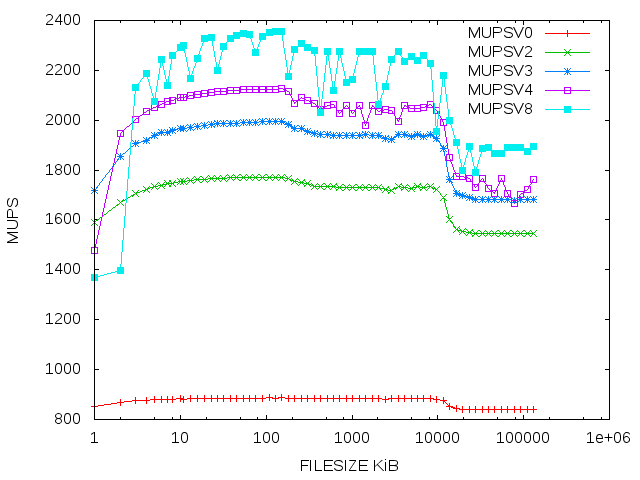
\includegraphics[scale=0.6]{pics/a3b.png}
	\caption{Plot of manual loop unrolling}
	\end{figure}
\end{center}

\subsection*{c)}
TODO

\section*{Aufgabe 4}
\subsection*{b)}

\begin{center}
	\begin{figure}[h]
	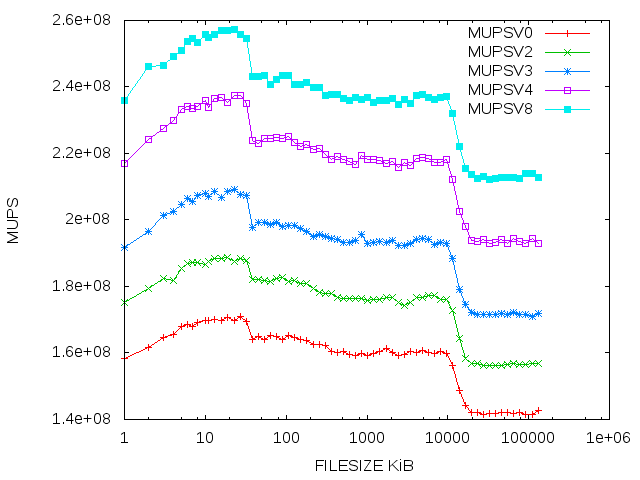
\includegraphics[scale=0.6]{pics/a4b.png}
	\caption{Plot of compiler based loop unrolling}
	\end{figure}
\end{center}

\subsection*{c)}
TODO

\end{document}
